\section{Part 1: Denoising of Simulated Data}

\begin{taskbox}[Part 1: introduction in the lab manual]
In this part we want to use the ICA method to study the removal of noise from a simulated EEG signal (the data of this part are in the folder \texttt{Lab2\_1}). Since the clean data (the desired signal) are available in the simulated signal, different algorithms can be evaluated and compared with quantitative metrics. For this purpose a 32-channel interictal (non-seizure) epileptic EEG signal is used. This realistic simulated data is the noise-free data (the desired signal), the matrix \texttt{X\_org}. A real signal containing muscle noise and background EEG is also given (\texttt{noise\_X}). We want to add the noise to the desired signal at different SNRs and then reconstruct the desired signal with blind source separation algorithms.
\end{taskbox}

\subsection*{Question 1: Plotting the clean signal}
\begin{taskbox}
Plot the noise-free signal \texttt{X\_org}. Label the channels and the time. You can use the files \texttt{plotEEG.m} and \texttt{eeg\_disp.m}. For a better display, you can tune the variable \texttt{offset} (the spacing between the signals shown for two channels).
\end{taskbox}

The matrix \texttt{X\_org} contains the desired 32-channel data. Figure~\ref{fig:xorg} shows all channels with their labels and the time axis. Sharp, few events can be seen on the background. According to the definition in the exercise, this data is simulated and interictal; no new clinical conclusion is inferred from it. For the stacked display, the mean of each channel was subtracted and a fixed vertical offset was added; this offset is only for display.

\begin{figure}[H]
\centering
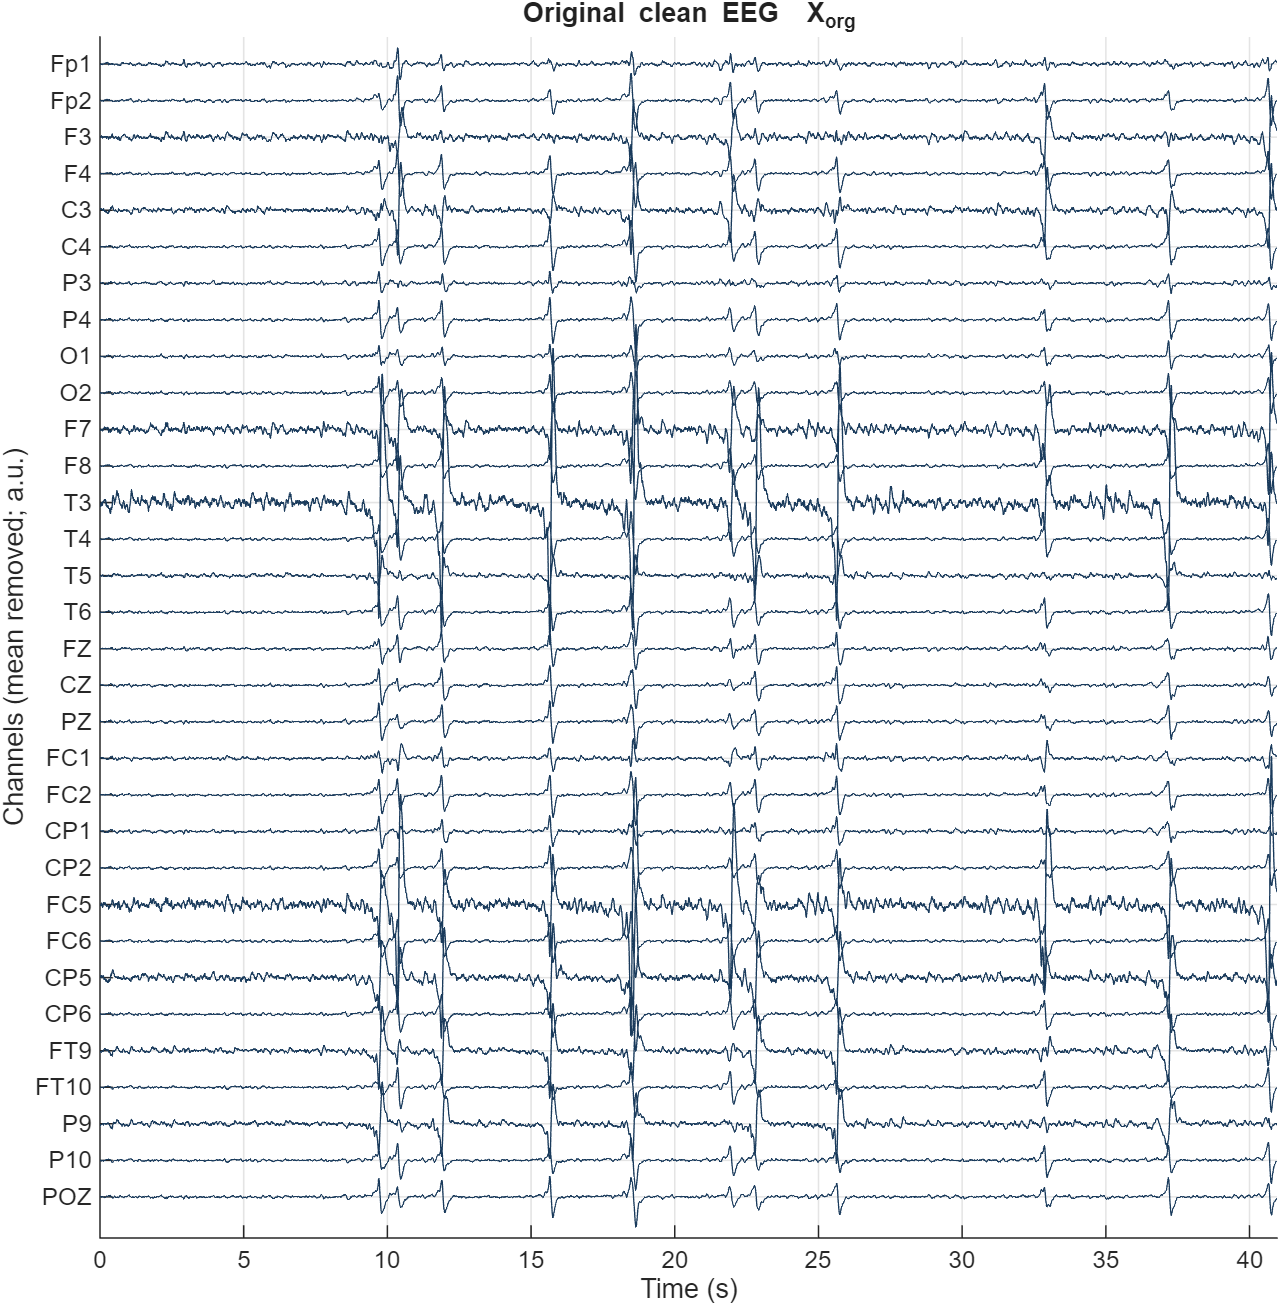
\includegraphics[width=0.85\textwidth,height=0.72\textheight,keepaspectratio]{fig01_clean_eeg_xorg.png}
\caption{The desired signal \texttt{X\_org} with the labels of all 32 channels and the time axis in seconds.}
\label{fig:xorg}
\end{figure}

\subsection*{Question 2: Examining the supplied noise}
\begin{taskbox}
Plot the noise \texttt{X\_noise}. Label the channels and the time.
\end{taskbox}

Figure~\ref{fig:xnoise} shows \texttt{X\_noise} itself, without multiplication by the noise coefficient. According to the exercise, this data contains background EEG and muscle contamination. The change of amplitude and the temporal envelope show that the noise is not necessarily stationary, and in some intervals faster and more clustered activity is seen. The noise should therefore not be assumed to be merely white Gaussian noise. Its contribution to the observation is determined after multiplication by a coefficient common to all channels.

\begin{figure}[H]
\centering
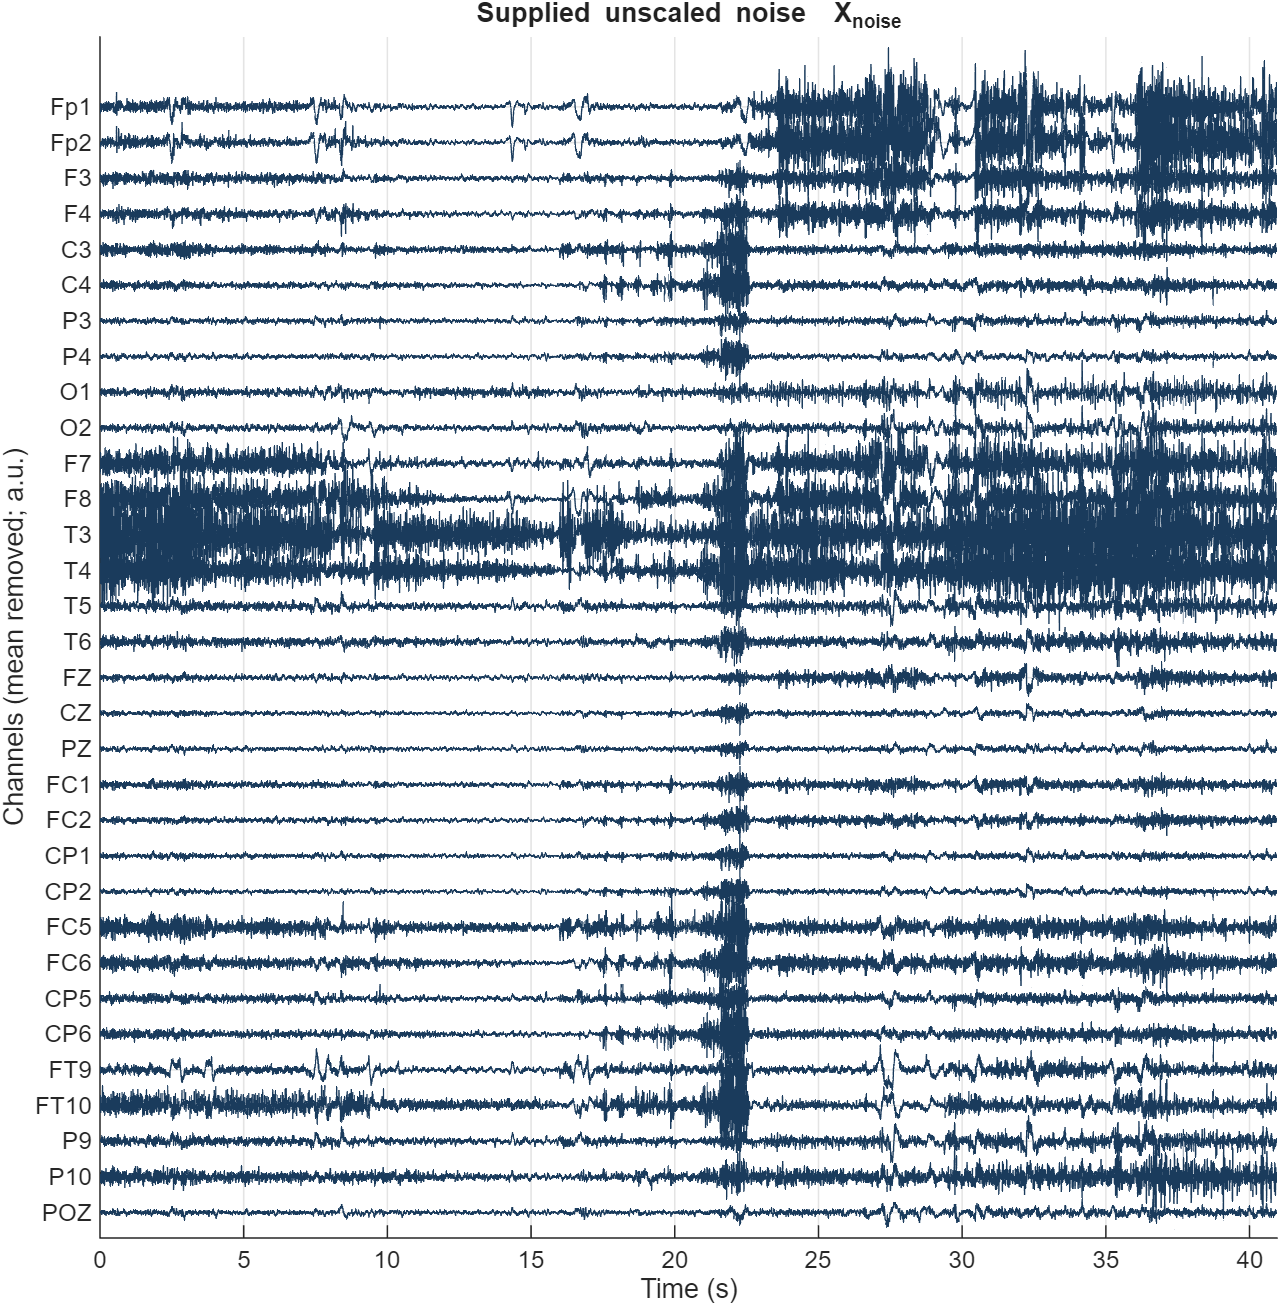
\includegraphics[width=0.85\textwidth,height=0.72\textheight,keepaspectratio]{fig02_noise_xnoise.png}
\caption{The raw noise \texttt{X\_noise} without scaling; the vertical spacing of the channels is only for readability.}
\label{fig:xnoise}
\end{figure}

\subsection*{Question 3: Building the observation at a specified SNR}
\begin{taskbox}
Add the noise to the original signal at different SNRs ($-5$~dB and $-15$~dB) and build the observation signal. Plot the noisy signal for $\mathrm{SNR}=-15$~dB and compare it with the noise-free signal. (The manual defines $\mathrm{SNR}_{dB}=10\log_{10}(P_{\mathrm{signal}}/P_{\mathrm{noise}})$; for a multichannel signal, $\mathbf{x}[m]=\mathbf{s}[m]+\sigma\mathbf{N}[m]$ with one $\sigma$ common to all channels, i.e.\ $\sigma^{2}=\frac{P_s}{P_N}\times10^{-\mathrm{SNR}_{dB}/10}$.)
\end{taskbox}

\begin{align}
X &= X_{\mathrm{org}}+\sigma X_{\mathrm{noise}}\\
\mathrm{SNR}_{dB} &= 10\log_{10}\!\left(\frac{\|X_{\mathrm{org}}\|_F^{2}}{\sigma^{2}\|X_{\mathrm{noise}}\|_F^{2}}\right)\\
\sigma &= \frac{\|X_{\mathrm{org}}\|_F}{\|X_{\mathrm{noise}}\|_F}\times10^{-\mathrm{SNR}_{dB}/20}
\end{align}

A common coefficient $\sigma$ was used for all channels. For an SNR of $-5$~dB, $\sigma$ equals 3.582232, and for $-15$~dB it equals 11.328013. The SNR measured after the addition was $-5$ and $-15$~dB, respectively. The ratio of the noise power to the desired-signal power in these two cases is about 3.16 and 31.62; the noise amplitude of the second case relative to the first is about $\sqrt{10}$ times larger.

\begin{lstlisting}[language=Matlab]
sigma = norm(X_org,'fro') / norm(X_noise,'fro') ...
        * 10^(-targetSNR/20);
X = X_org + sigma * X_noise;
\end{lstlisting}

Figure~\ref{fig:noisy15} shows the $-15$~dB observation. As the noise increases, identifying the desired events becomes more difficult in many channels. The exact comparison of amplitudes is made in the overlaid figures of channels 13 and 24; the vertical spacing of the stacked plots alone is not a measure of the SNR.

\begin{figure}[H]
\centering
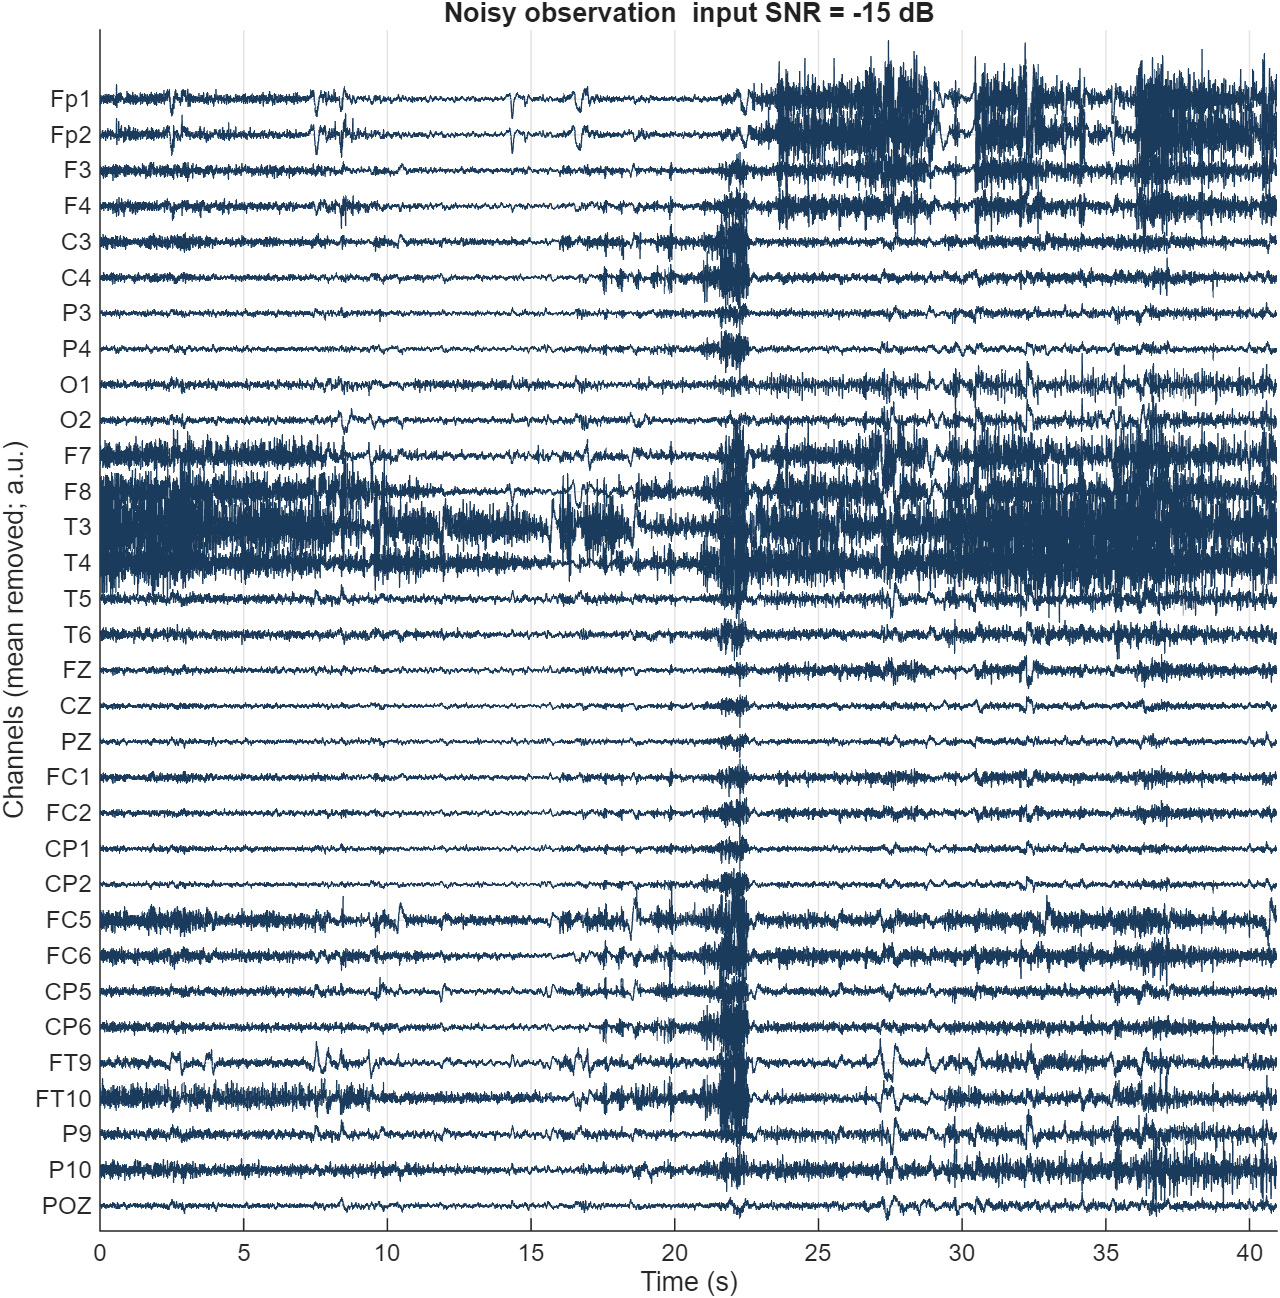
\includegraphics[width=0.85\textwidth,height=0.72\textheight,keepaspectratio]{fig03_noisy_observation_m15db.png}
\caption{The noisy observation at an SNR of $-15$~dB; all channels are labeled.}
\label{fig:noisy15}
\end{figure}

\subsection*{Questions 4 and 5: Separation and selection of the sources}
\begin{taskbox}
\textbf{4.} Extract the sources using an ICA method of your choice. You can use the function \texttt{R2COM.m} (the R2Com algorithm).\\
\textbf{5.} Examine all the obtained sources, keep the desired sources (spiky sources), and remove the other sources.
\end{taskbox}

For each SNR, the COM2R algorithm was run separately on the mean-removed observation, which has full rank. The size of $A$ and $W$ is $32\times32$ and the size of $S$ is $32\times10240$. All components were examined in time, frequency and mixing weights; the complete sheets are given in Appendix~C. The IC numbers of the two SNRs belong only to their own decomposition and must not be assumed to correspond one to one.

\begin{lstlisting}[language=Matlab]
channelMean = mean(X,2);
Xc = X - channelMean;
[A,W,sweeps] = COM2R(Xc,32);
S = W * Xc;
\end{lstlisting}

For a transparent and reproducible record of the selection of the spiky sources, the following three simultaneous conditions were used. The thresholds are an instructional, data-specific rule and are not a boundary for medical diagnosis. \texttt{X\_org} was not used to tune these selections; it served only as the reference for computing the error and comparing the figures.
\begin{equation}
\kappa\ge 6;\qquad \max_t|z(t)|\ge 6;\qquad \mathrm{HF}\le 0.20
\end{equation}

\begin{center}
\begin{tabular}{@{}lcc@{}}
\toprule
\textbf{Input SNR} & \textbf{Kept components} & \textbf{Kept / removed}\\
\midrule
$-5$ dB  & 2\ 5\ 9\ 10\ 12\ 21\ 23\ 32 & 8 / 24\\
$-15$ dB & 7\ 8\ 18\ 20\ 30\ 32        & 6 / 26\\
\bottomrule
\end{tabular}
\end{center}

Kurtosis alone is not sufficient: for example, at $-5$~dB component 6, with a kurtosis of about 109.6 and a high-frequency share of about 0.778, was removed; despite its sharpness and high kurtosis, its activity is a high-frequency burst. Conversely, keeping a component with a sharp event does not guarantee that the component is completely free of background or noise. The large error of the $-15$~dB case shows the limitation of this very separation and of the selection rule.

In this part, the aim of the exercise is to keep the spiky sources and set aside the other sources. In the real-data part, the aim is to preserve the brain components and remove only those with artifactual evidence; the selection rule of the simulation was therefore not generalized to the real data.

\subsection*{Questions 6 and 7: Reconstruction and comparison of the channels}
\begin{taskbox}
\textbf{6.} Project the desired sources back to the sensor domain (the observation domain) and build the denoised observations (\texttt{X\_den}).\\
\textbf{7.} Plot the denoised observations for channels 13 and 24 together with the original noise-free data and the noisy data.
\end{taskbox}

\begin{equation}
X_{\mathrm{den}}=A(:,K)\,S(K,:)+\mu\mathbf{1}^{T}
\end{equation}
After selecting the set $K$, i.e.\ \texttt{SelSources}, only the contribution of those components was returned to the sensor space. The mean term was added because of the earlier mean removal, and it is consistent with the exercise formula for mean-removed data. Channel 13 in this data is T3 and channel 24 is FC5. At $-5$~dB, the reconstruction follows many of the reference events, but differences in the background and in the amplitude remain.

\begin{figure}[H]
\centering
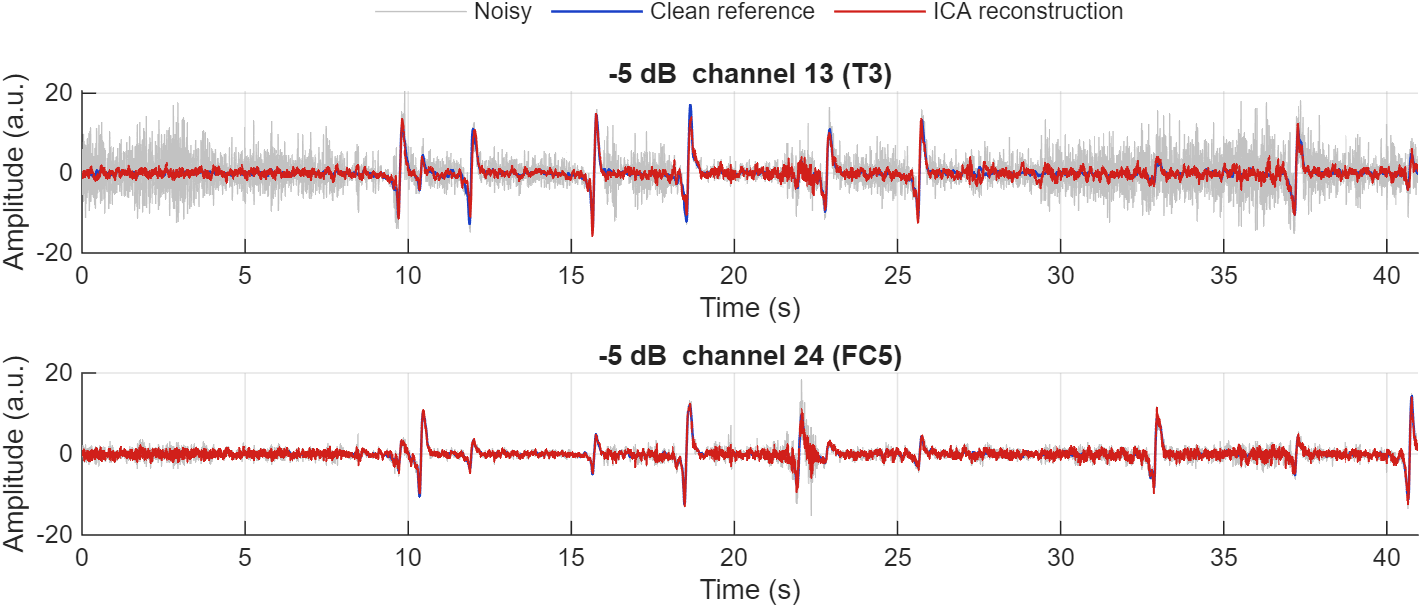
\includegraphics[width=\textwidth]{fig04_channels_t3_fc5_m5db.png}
\caption{Comparison of channels T3 and FC5 at $-5$~dB; gray is the observation, blue is the clean reference and red is the reconstruction.}
\label{fig:ch5}
\end{figure}

\begin{figure}[H]
\centering
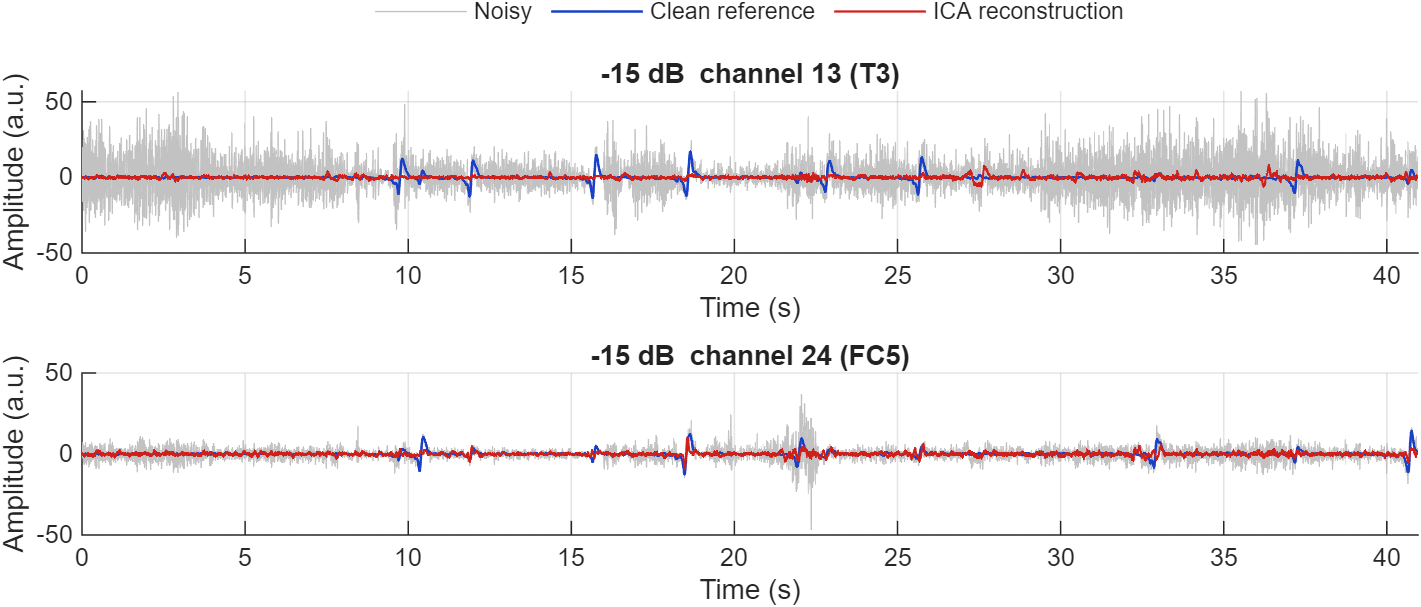
\includegraphics[width=\textwidth]{fig05_channels_t3_fc5_m15db.png}
\caption{The same comparison at $-15$~dB; part of the reference spikes, especially in T3, has not been recovered well.}
\label{fig:ch15}
\end{figure}

\paragraph{Temporal detail and error of the selected channels.} The zooms are shown around the largest reference event of channel 13; the location of the zoom was not used to select the components. Under strong noise, an apparent smoothing of the output does not necessarily mean preservation of the desired event. Both the waveform shape and the numerical error must be examined.

\begin{figure}[H]
\centering
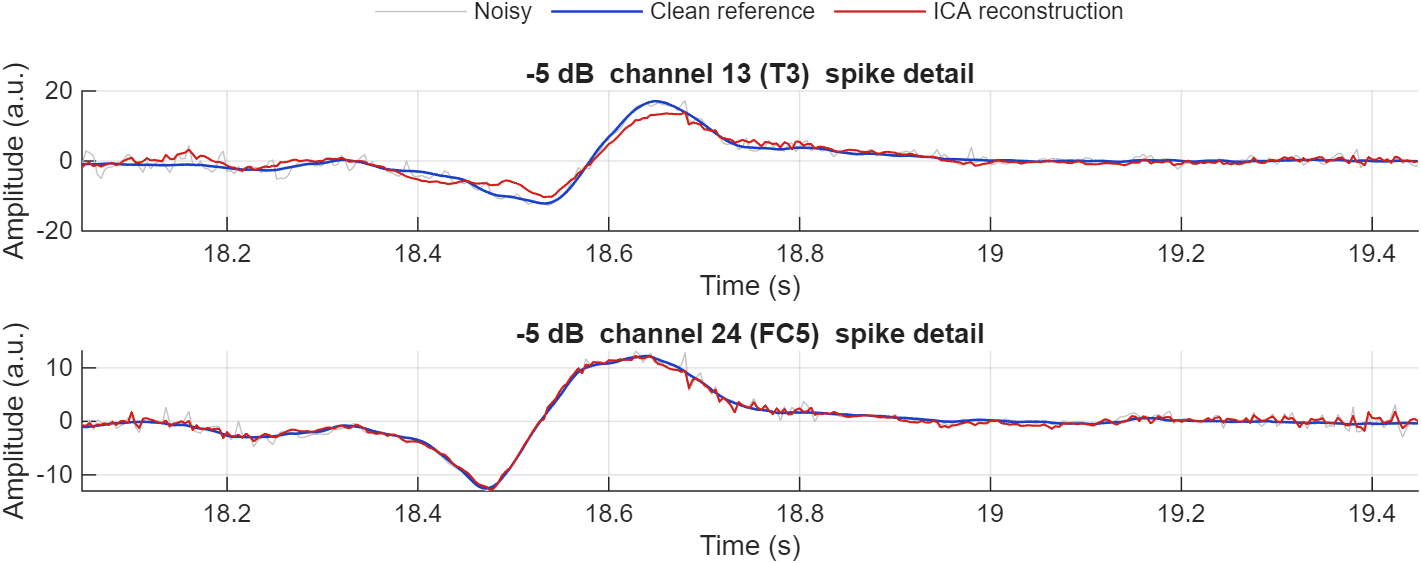
\includegraphics[width=0.95\textwidth]{fig06_event_detail_m5db.png}
\caption{Detail of an event at $-5$~dB; comparison of the shape and amplitude of the reconstruction with the reference.}
\label{fig:det5}
\end{figure}

\begin{figure}[H]
\centering
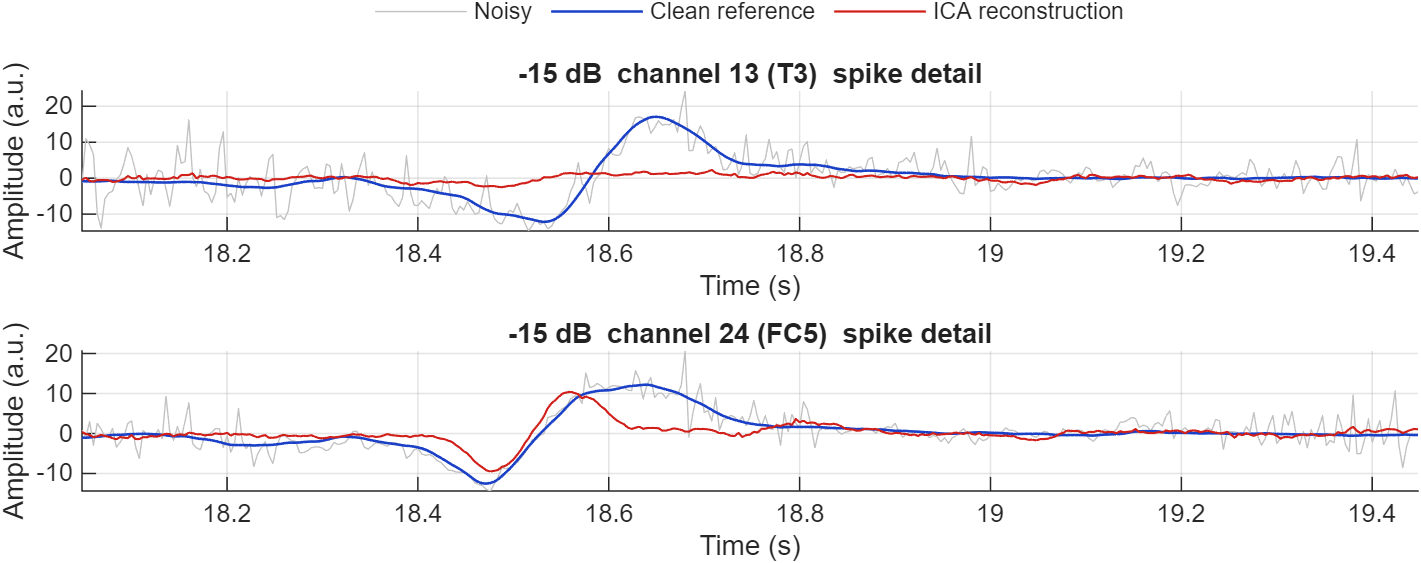
\includegraphics[width=0.95\textwidth]{fig07_event_detail_m15db.png}
\caption{Detail of the same interval at $-15$~dB; the difference between the reconstruction and the reference is more evident.}
\label{fig:det15}
\end{figure}

\begin{center}
\begin{tabular}{@{}clcc@{}}
\toprule
\textbf{SNR} & \textbf{Channel} & \textbf{Input RRMSE} & \textbf{Output RRMSE}\\
\midrule
$-5$ dB  & 13 T3  & 1.442288 & 0.416973\\
$-5$ dB  & 24 FC5 & 0.581928 & 0.367643\\
$-15$ dB & 13 T3  & 4.560914 & 1.044193\\
$-15$ dB & 24 FC5 & 1.840218 & 0.963348\\
\bottomrule
\end{tabular}
\end{center}

\subsection*{Question 8: Computing and analyzing the RRMSE}
\begin{taskbox}
Compute the RRMSE (relative RMSE) for each SNR. Analyze the obtained results. (The manual defines $\mathrm{RRMSE}=\sqrt{\sum_{n=1}^{32}\sum_{t=1}^{T}(x_{org}^{(n)}(t)-x_{den}^{(n)}(t))^2}\big/\sqrt{\sum_{n=1}^{32}\sum_{t=1}^{T}(x_{org}^{(n)}(t))^2}$.)
\end{taskbox}

\begin{align}
\mathrm{RRMSE}&=\frac{\|X_{\mathrm{org}}-X_{\mathrm{den}}\|_F}{\|X_{\mathrm{org}}\|_F}\\
\mathrm{SNR}_{\mathrm{out}}&=-20\log_{10}(\mathrm{RRMSE})
\end{align}
The RRMSE is the ratio of the Frobenius norm of the error to the Frobenius norm of the reference, and it is computed from the sum over the samples and the channels; this value is not the mean RRMSE of the channels. The relation of the output SNR to the RRMSE also holds with this same reference and the same definition of the error.

\begin{center}
\small
\begin{tabular}{@{}cccccc@{}}
\toprule
\textbf{Input SNR} & $\sigma$ & \textbf{Input RRMSE} & \textbf{Output RRMSE} & \textbf{Output SNR} & \textbf{SNR improvement}\\
\midrule
$-5$ dB  &  3.582232 & 1.778279 & 0.714724 &  2.9172 dB & 7.9172 dB\\
$-15$ dB & 11.328013 & 5.623413 & 2.084281 & $-6.3791$ dB & 8.6209 dB\\
\bottomrule
\end{tabular}
\end{center}

\begin{figure}[H]
\centering
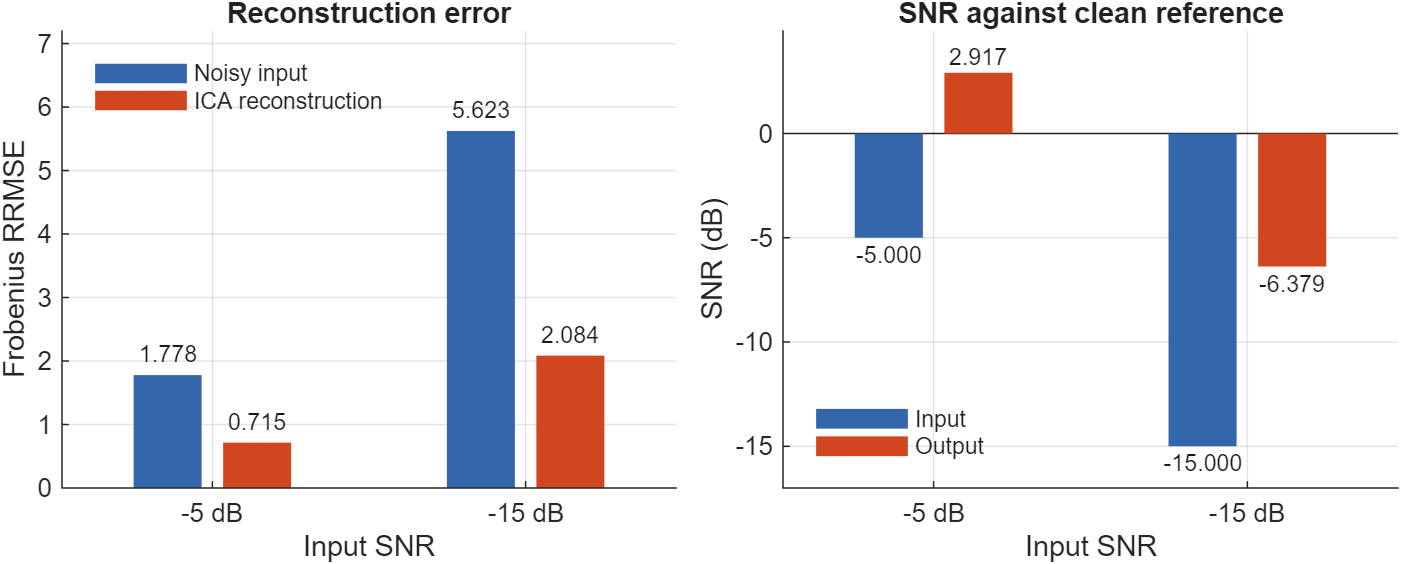
\includegraphics[width=0.95\textwidth]{fig08_rrmse_and_snr.png}
\caption{Comparison of the relative error and the SNR; both cases improve relative to the observation, but the absolute quality of the $-15$~dB case is lower.}
\label{fig:rrmse}
\end{figure}

The relative reduction of the error norm with respect to the input is about 59.8 percent and 62.9 percent. These percentages are not ``accuracy'' or ``percent of the signal recovered.'' In the $-15$~dB case, the output RRMSE is 2.084 and the output SNR is still $-6.379$~dB; the residual error energy is about 4.34 times the energy of the clean reference. For comparison, an all-zero estimate has an RRMSE of one. Consequently, the improvement relative to the very noisy observation is not sufficient to consider the reconstruction of this case adequate.

This result is consistent with the presence of mixed sources, the dominance of noise, and the loss or attenuation of some spikes. The larger improvement in dB in the noisier case must not be confused with the output being better. Tuning the selections by using the clean reference directly could have reduced the error of the same data, but it would have made the evaluation of blind separation optimistic; such tuning was not performed.

\paragraph{Spectral examination of the simulation reconstruction.} Figure~\ref{fig:psdsim} shows the mean PSD of the channels at the two SNRs.

\begin{figure}[H]
\centering
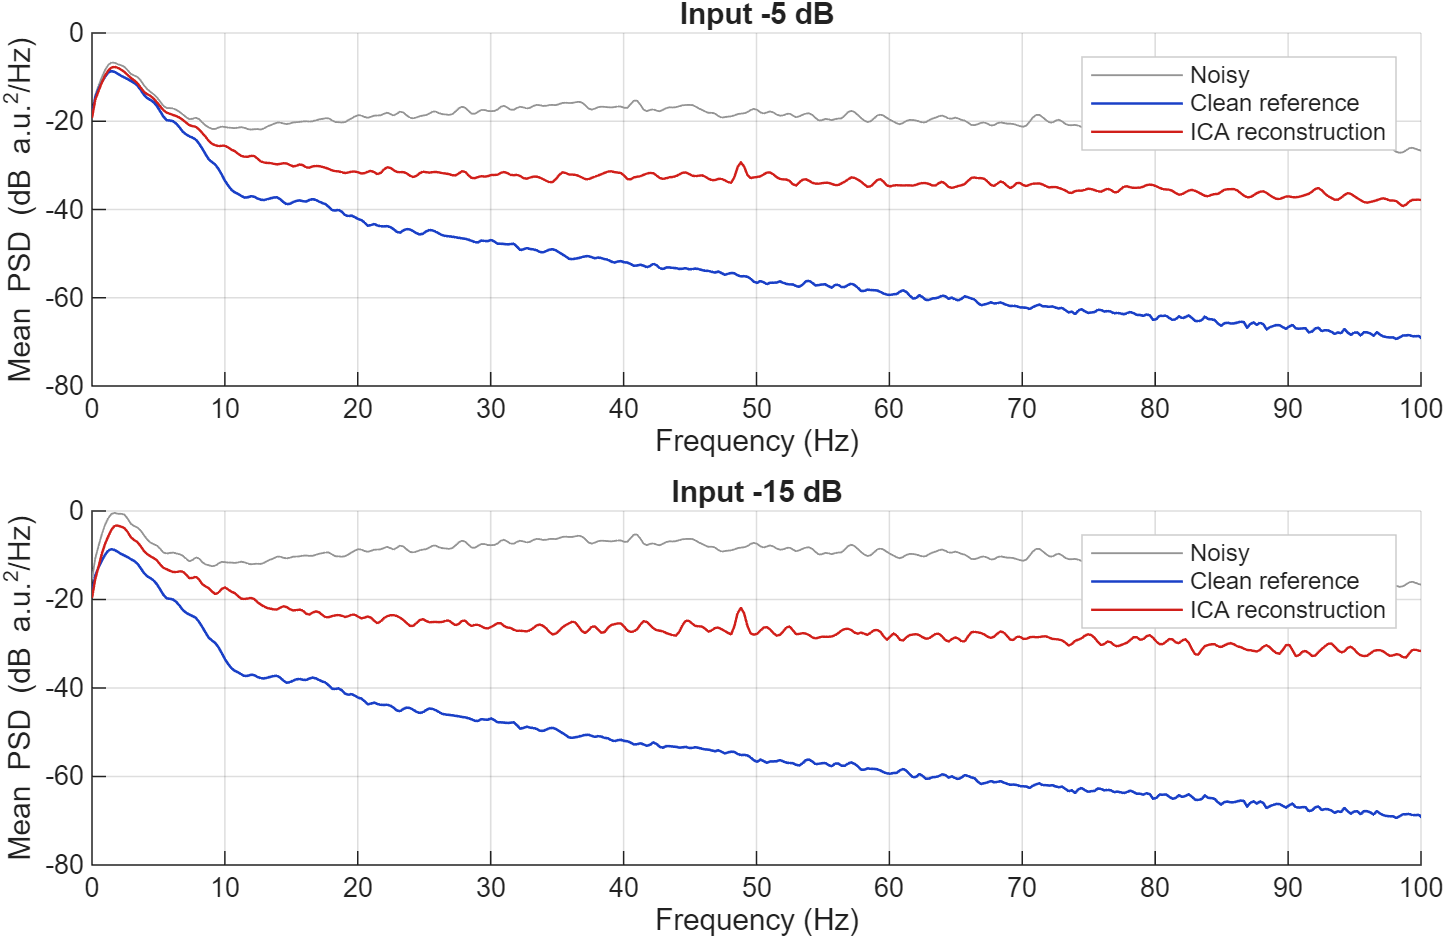
\includegraphics[width=0.9\textwidth]{fig09_psd_simulation.png}
\caption{Mean PSD of the channels at the two SNRs; a decrease of high-frequency power alone does not prove preservation of the spike shape.}
\label{fig:psdsim}
\end{figure}

The PSD plot shows that the reconstruction has reduced a considerable share of the observation power, especially at higher frequencies. However, the PSD does not completely preserve the information on the phase and the exact timing of events. Two signals with similar spectra can have different temporal shapes; spectral analysis was therefore used alongside the waveform and the RRMSE.

The residual of the reconstruction using all components was about $3.87\times10^{-12}$ and $4.69\times10^{-12}$. These small values confirm the consistency of the matrices $A$ and $W$ and of the back-mapping; they do not prove complete statistical independence, the biological correctness of the components, or the quality of the noise removal.
